% Appendix A

\chapter{Questionnaires}
\label{an:questionnaires}

%----------------------------------------------------------------------------------------

\noindent This appendix contains screenshots of both the initial (before translating) and final (after translating) questionnaires that were given to the study's participants. For further details on the design of the questionnaires, please refer to \autoref{ch:questionnaires}.

\paragraph{Please Note:} Form navigation and interface elements, such as the ``Next'' and ``Submit'' buttons and ``Required*'' field, were shown in the language participants have their Google account set up in or, if they don't have one, in the browser's default language. The screenshots in this chapter show the navigation and interface elements in Swedish, but this varied for each participant.

%----------------------------------------------------------------------------------------

\section{Initial Questionnaire}

\subsection{Questions}

\graffito{Note: in case of closed questions, the possible options are shown in square brackets.}

\begin{enumerate}
\item What does translation mean to you? 
\item What is your gender? [Male, Female, Other]
\item What is your year of birth? 
\item What is your current occupation?
\item Which language(s) are you native in? [English, Spanish, French, German, Catalan, Basque, Galician, Chinese, Japanese, Portuguese, Italian, Russian, Greek, Other]
\item Which other language(s) do you speak? [English, Spanish, French, German, Catalan, Basque, Galician, Chinese, Japanese, Portuguese, Italian, Russian, Greek, Other]
\item Have you studied translation? [Yes, No]
\item If yes, for how many years have you studied translation?
\item Have you worked as a translator? [Yes, No]
\item If yes, for how many years have you worked as a translator?
\item Do you have professional experience working on the following translation-related tasks? [Multiple choices can be selected] [Translating from scratch, Proof-reading, Machine translation post-editing, Transcreation, Loclalizing, Managing terminology, Setting-up style guides, Translating with a CAT tool (For example, Trados), Preparing documents for internationalisation, Machine translation system setup (for example, Moses SMT), Machine translation quality evaluation]
\item What do you think are the most INTERESTING tasks to carry out when translating?
\item What do you think are the most BORING tasks to carry out when translating?
\item If a tool could be created to automate any task you carry out when translating so you don't have to do it, which task would it be?
\item How important are the following considerations when translating? [Very important (1), (2), (3), (4), Not at all important (5)]
\begin{enumerate}
\item Accurately portraying the source text
\item Applying a style guide consistently
\item Using terminology consistently
\item Providing a grammatically correct translation
\item Conforming to what the client requests in the translation brief
\item Providing a fluent translation/idiomatic translation
\end{enumerate}
\item Which of the previous considerations do you prioritise the most? [Accurately portraying the source text, Applying a style guide consistently, Using terminology consistently, Providing a grammatically correct translation, Conforming to what the client requests in the translation brief, Providing a fluent translation/idiomatic translation]
\item Are there any other considerations you usually take into account?
\item Do you usually use glossaries / terminological lists when translating? [Yes, No]
\item Do you usually use style guides when translating? [Yes, No]
\item Do you usually use computer-aided translation (CAT) when translating? [Yes, No]
\item Do you agree with the following statements? [Strongly agree (1), (2), (3), (4), Strongly Disagree (5)]
\begin{enumerate}
\item Machine translation is useful for translators
\item Machine translation is ONLY useful for the general public
\item Machine translation will one day replace human translators
\item Machine translation today provides good quality translations
\item It is difficult to understand how machine translation works
\item I would like to learn more about machine translation
\end{enumerate}
\item Do you think your translations are better than those from machine translation? [Yes, No]
\item Why?
\end{enumerate}

\subsection{Screenshots}

\noindent The following are screenshots of the questionnaire that participants had to fill in before starting the translation tasks.

\begin{figure}[H]
\myfloatalign
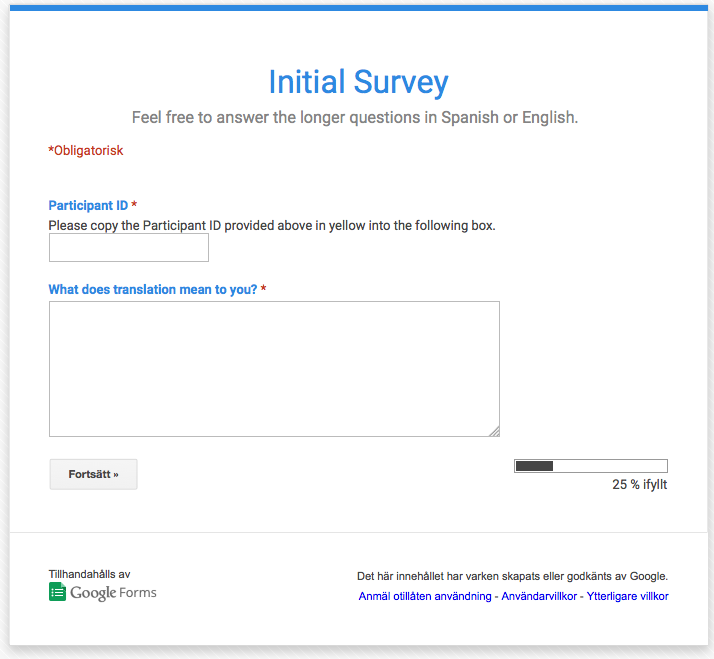
\includegraphics[width=\textwidth]{img/initial_questionnaire/initial_1.png}
\caption{Initial Questionnaire (Page 1)}
\end{figure}

\begin{figure}[H]
\myfloatalign
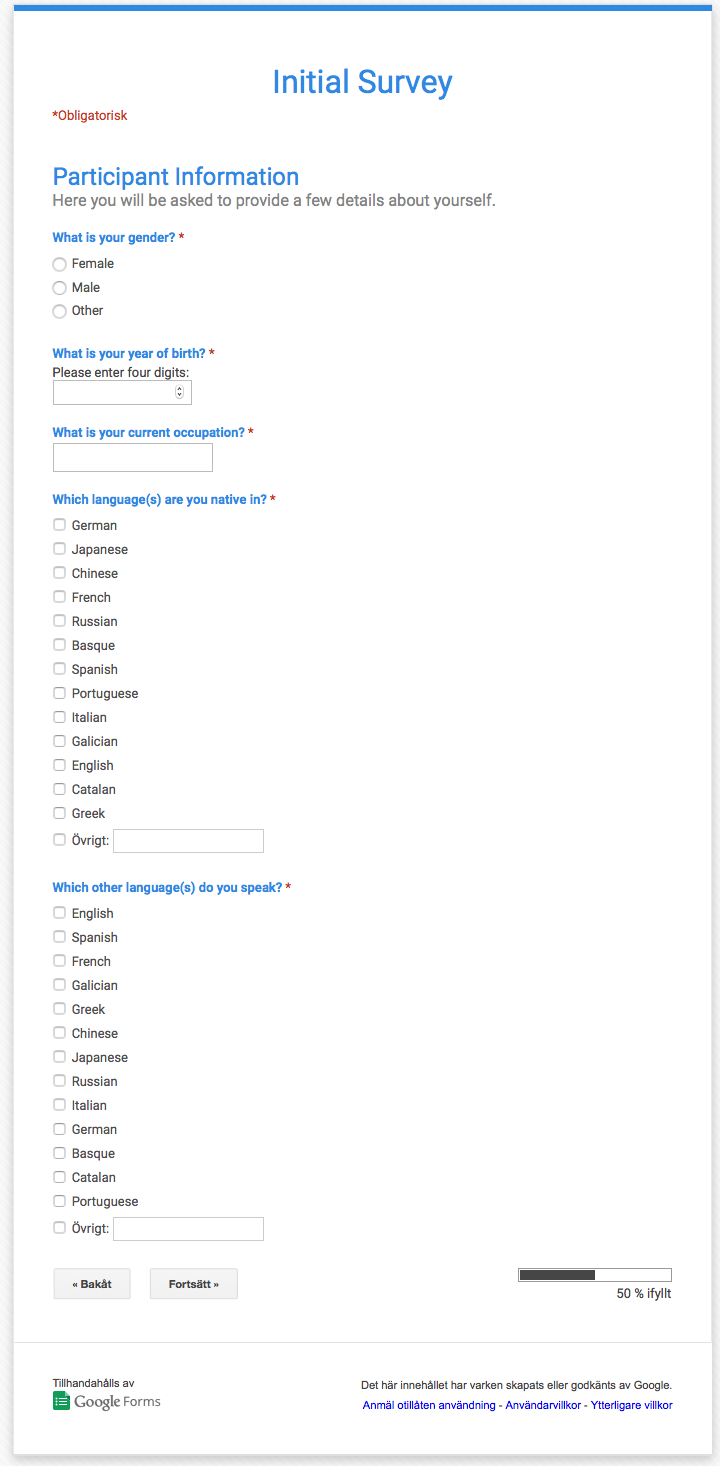
\includegraphics[height=\textheight]{img/initial_questionnaire/initial_2.png}
\caption{Initial Questionnaire (Page 2)}
\end{figure}

\begin{figure}[H]
\myfloatalign
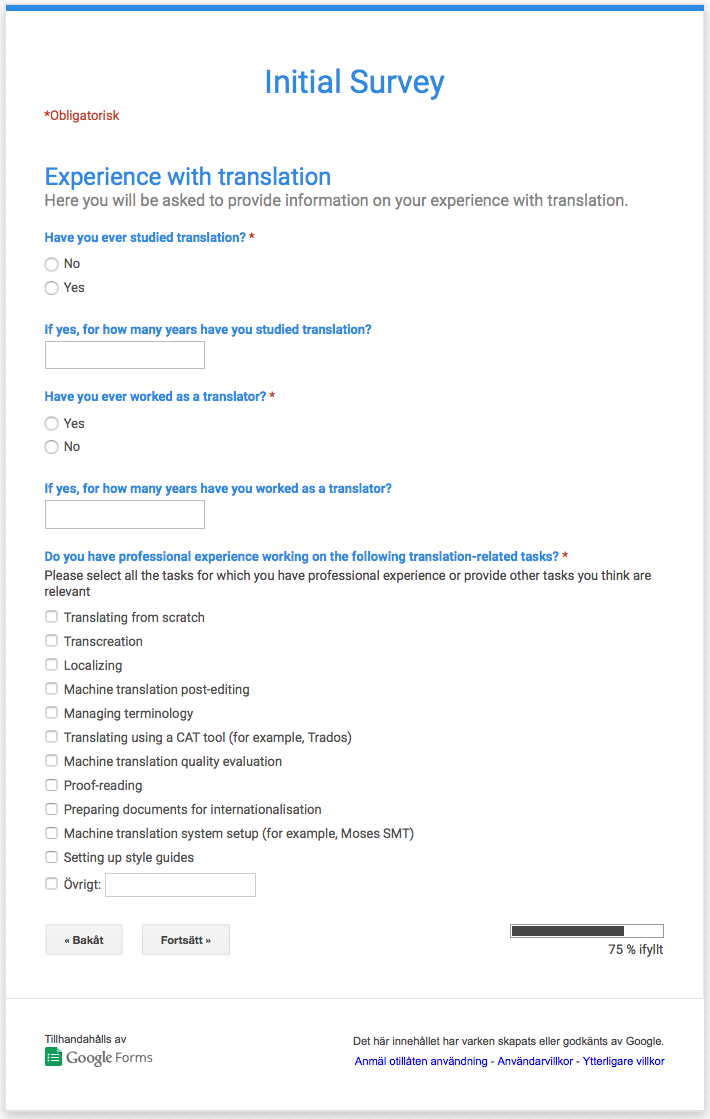
\includegraphics[width=\textwidth]{img/initial_questionnaire/initial_3.png}
\caption{Initial Questionnaire (Page 3)}
\end{figure}

\begin{figure}[H]
\myfloatalign
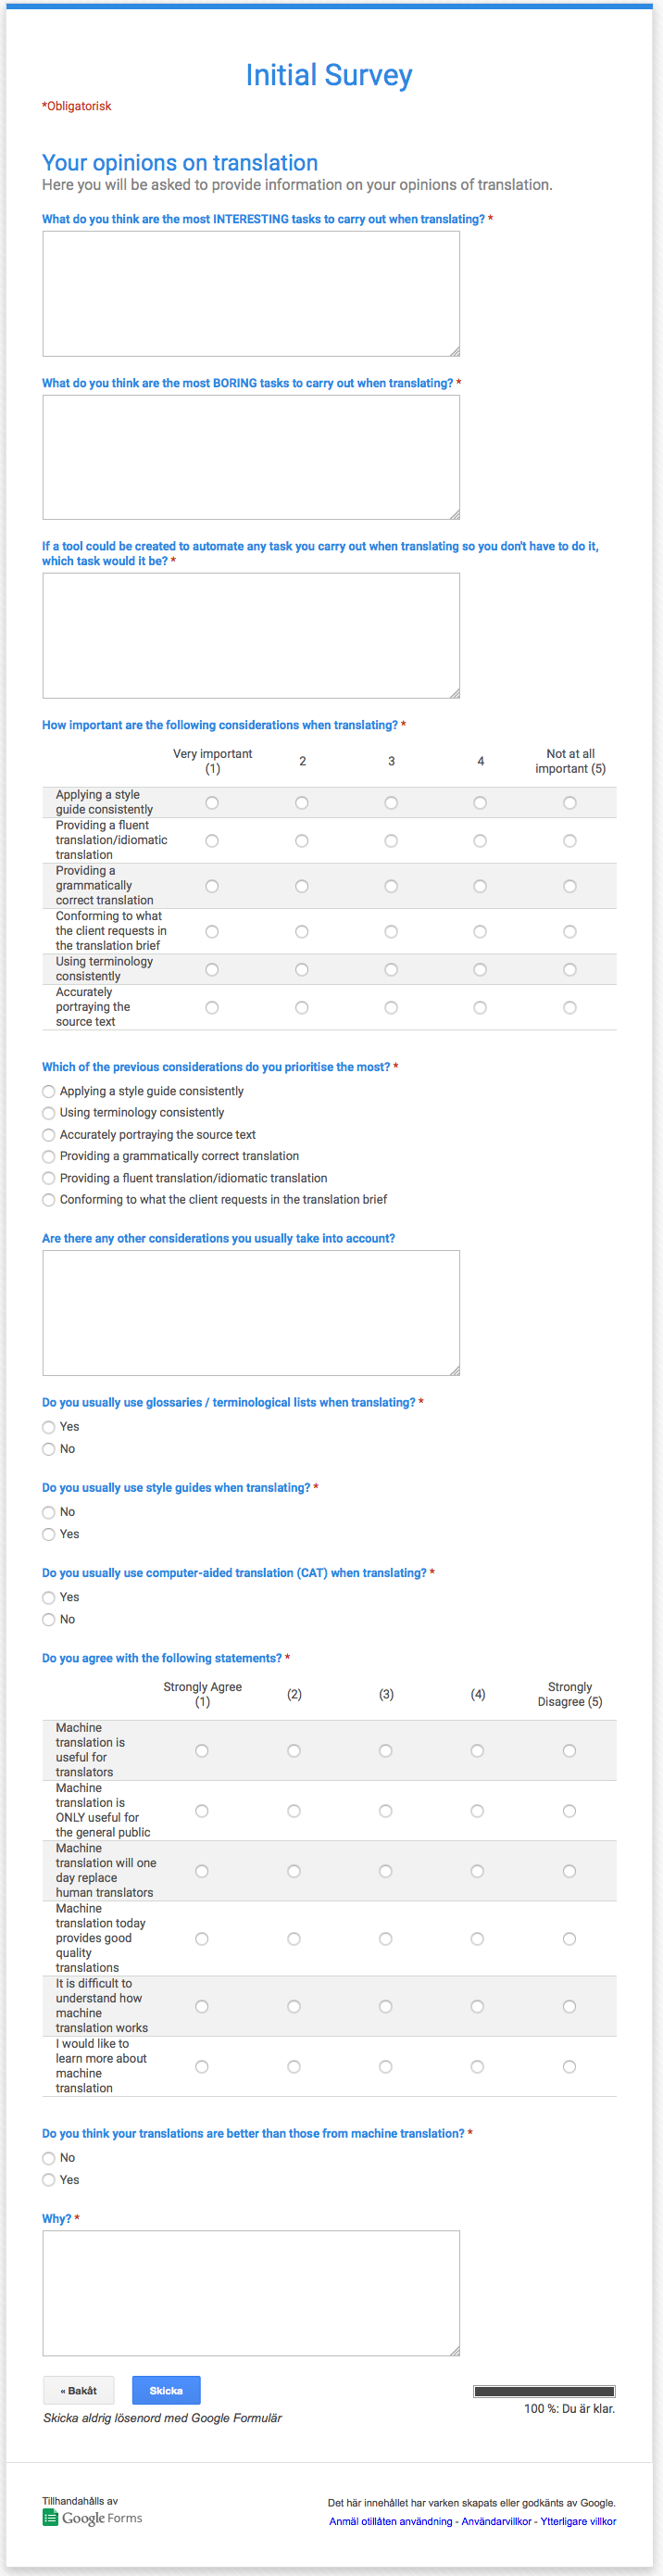
\includegraphics[height=\textheight]{img/initial_questionnaire/initial_4.png}
\caption{Initial Questionnaire (Page 3)}
\end{figure}

\newpage
%----------------------------------------------------------------------------------------

\section{Final Questionnaire}

\subsection{Questions}

\graffito{Note: in case of closed questions, the possible options are shown in square brackets.}

\begin{enumerate}
    \item After reading the translation brief, did you establish any priorities and restrictions for the translation? [Yes, No]
    \item If yes, which ones?
    \item Which translation was the hardest? [Text 1, Text 2, Text 3]
    \item Why was it hard?
    \item Which translation was the easiest? [Text 1, Text 2, Text 3]
    \item Why was it easy?
    \item During which translation did you feel you had MOST control over your final translation? [Text 1, Text 2, Text 3]
    \item Why did you feel in control?
    \item During which translation did you feel you had LEAST control over your final translation? [Text 1, Text 2, Text 3]
    \item Why did you not feel in control?
    \item Approximately, how many minutes do you think it took you to translate Text 1?
    \item What did you LIKE the most about translating Text 1?
    \item What did you DISLIKE the most about translating Text 1?
    \item Overall, how satisfied were you with the task of translating Text 1? [Very satisfied, Somewhat satisfied, Neutral, Somewhat dissatisfied, Very dissatisfied]
    \item Overall, how satisfied were you with the quality of your final translation of Text 1? [Very satisfied, Somewhat satisfied, Neutral, Somewhat dissatisfied, Very dissatisfied]
    \item Do you have any additional comments on the translation of Text 1?
    \item Approximately, how many minutes do you think it took you to translate Text 2?
    \item What did you LIKE the most about translating Text 2?
    \item What did you DISLIKE the most about translating Text 2?
    \item How would you rate the quality of the machine translation suggestions? [Well below average, Below average, Average, Above average, Well above average]
        \begin{enumerate}
            \item Grammaticality
            \item Style
            \item Accuracy
        \end{enumerate}
    \item Would you have preferred to translate from scratch without the machine translation suggestions? [Yes, No]
    \item Overall, how satisfied were you with the task of translating Text 2? [Very satisfied, Somewhat satisfied, Neutral, Somewhat dissatisfied, Very dissatisfied]
    \item Overall, how satisfied were you with the quality of your final translation of Text 2? [Very satisfied, Somewhat satisfied, Neutral, Somewhat dissatisfied, Very dissatisfied]
    \item Do you have any additional comments on the translation of Text 2?
    \item Approximately, how many minutes do you think it took you to translate Text 3?
    \item What did you LIKE the most about translating Text 3?
    \item What did you DISLIKE the most about translating Text 3?
    \item Did you consult the Wikipedia Style Guide linked to in the Translation Brief? [Yes, No]
    \item Why?
    \item Do you agree with the following statements? [Strongly agree (1), (2), (3), (4), Strongly Disagree (5)]
        \begin{enumerate}
            \item The style hints were helpful
            \item There were too many style hints
            \item The style hints were easy to understand
            \item The style hints were too long
            \item The boxes where the style hints were shown were distracting
            \item The style hints contained wrong information
        \end{enumerate}
    \item Would you have preferred to translate from scratch without the style suggestions? [Yes, No]
    \item Overall, how satisfied were you with the task of translating Text 3? [Very satisfied, Somewhat satisfied, Neutral, Somewhat dissatisfied, Very dissatisfied]
    \item Overall, how satisfied were you with the quality of your final translation of Text 3? [Very satisfied, Somewhat satisfied, Neutral, Somewhat dissatisfied, Very dissatisfied]
    \item Do you have any additional comments on the translation of Text 3?
    \item Do you have any final comments about any aspect of the experiment?
\end{enumerate}

\subsection{Screenshots}

\noindent The following are screenshots of the questionnaire that participants had to fill in after completing the translation tasks. Participants were shown a reminder (not seen in the following screeenshots) of the source texts they had translated to help job their memory.

\begin{figure}[h]
\myfloatalign
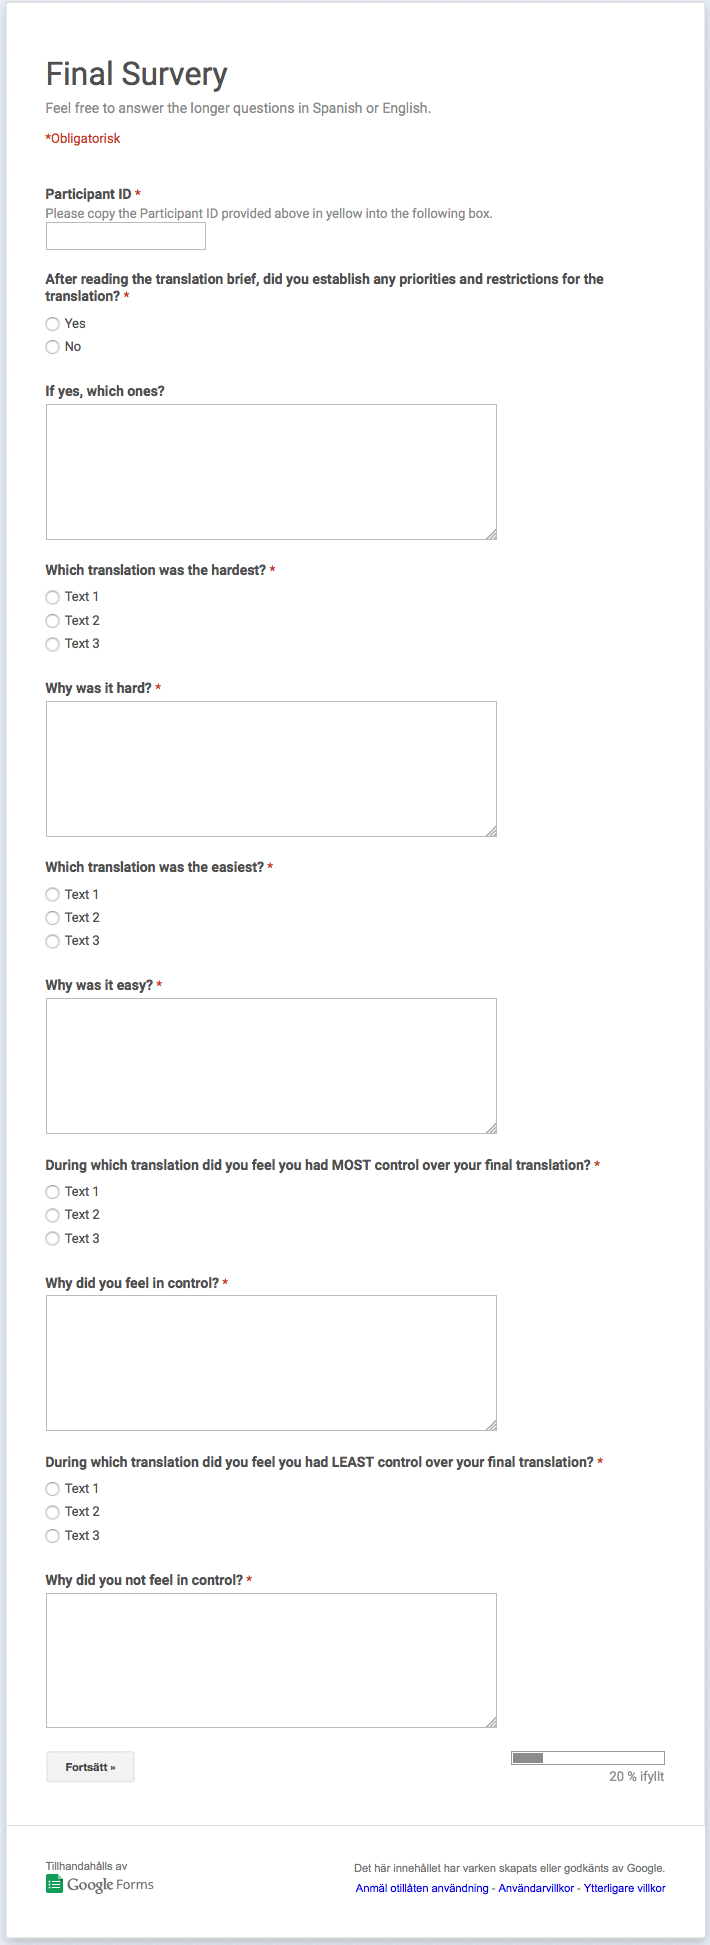
\includegraphics[height=\textheight]{img/final_questionnaire/final_1.png}
\caption{Final Questionnaire (Page 1)}
\end{figure}

\begin{figure}[h]
\myfloatalign
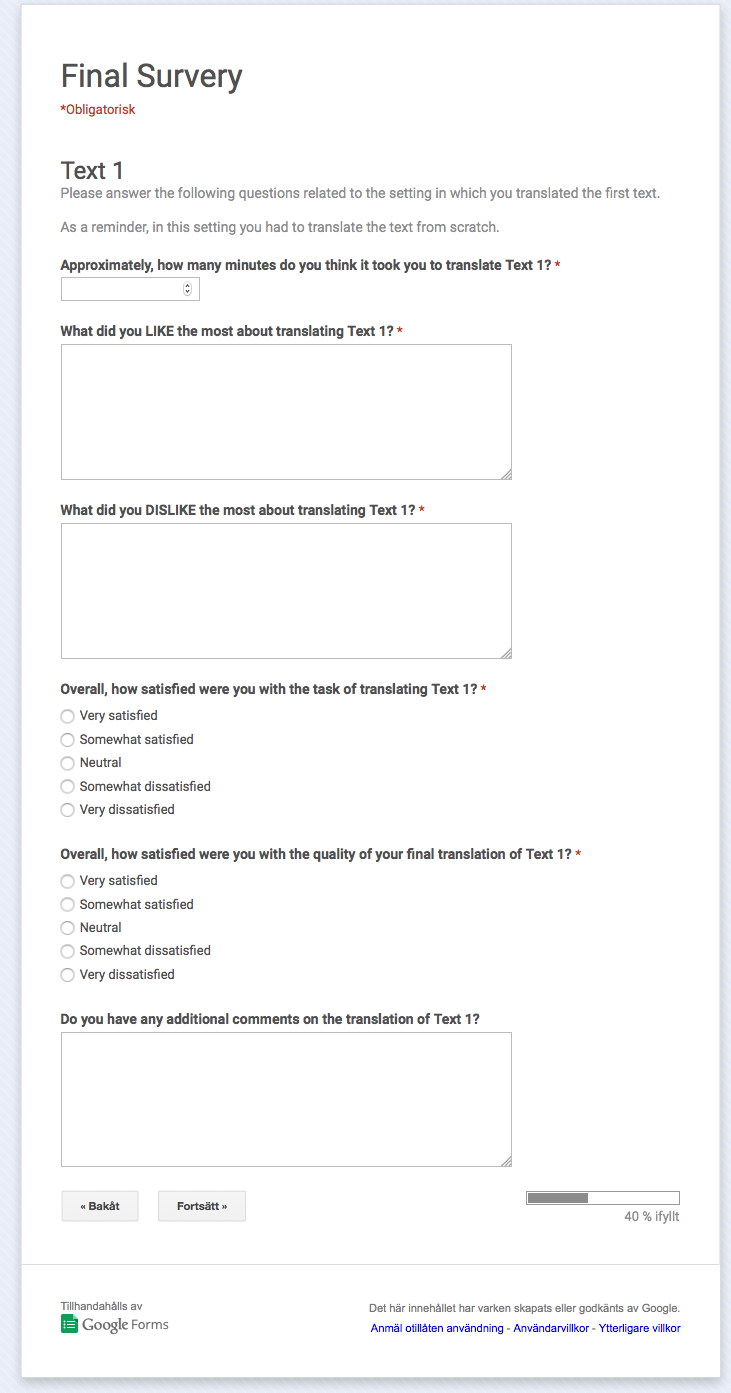
\includegraphics[height=\textheight]{img/final_questionnaire/final_2.png}
\caption{Final Questionnaire (Page 2)}
\end{figure}

\begin{figure}[h]
\myfloatalign
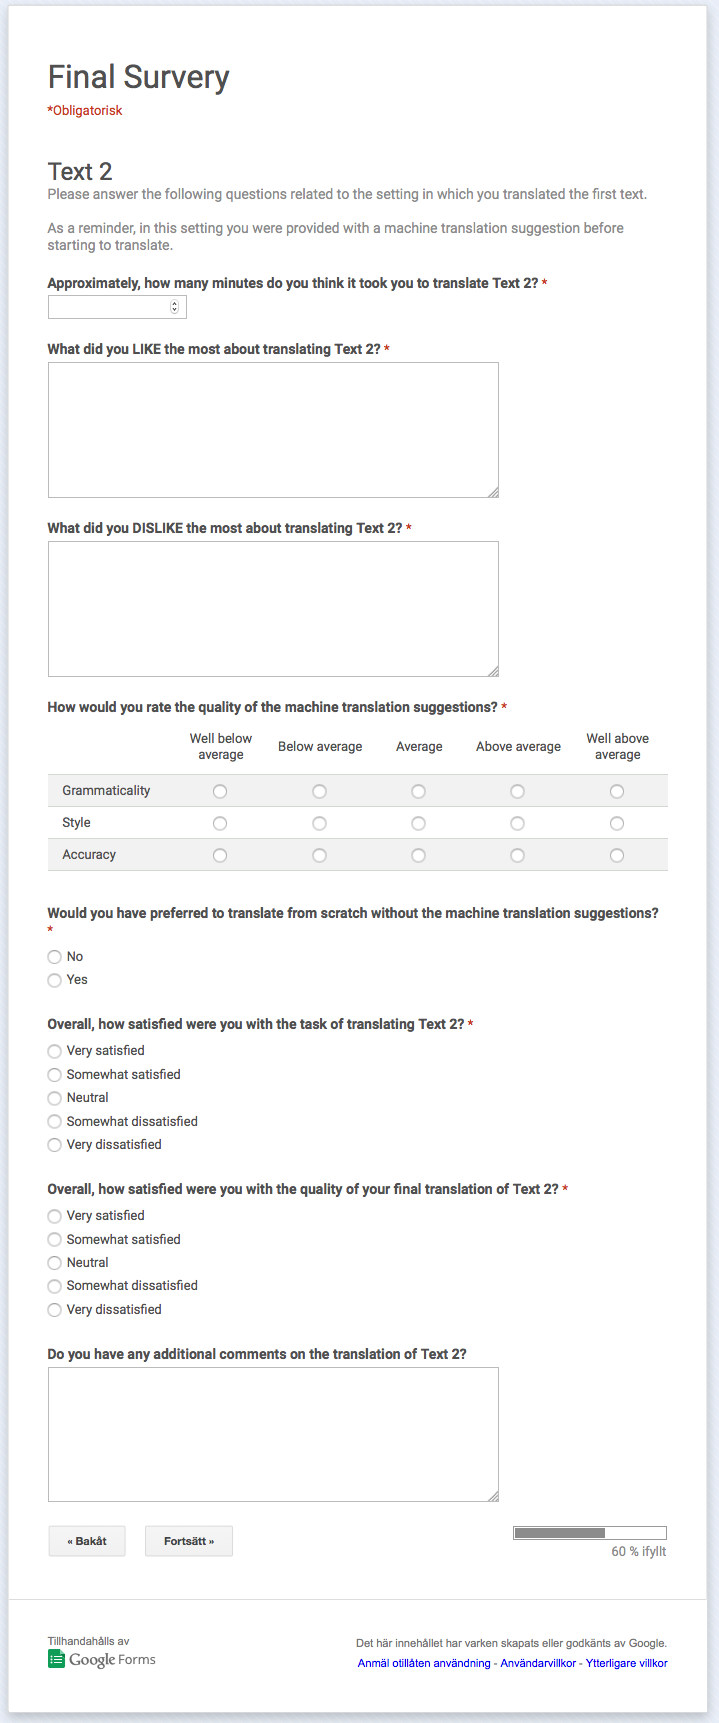
\includegraphics[height=\textheight]{img/final_questionnaire/final_3.png}
\caption{Final Questionnaire (Page 3)}
\end{figure}

\begin{figure}[h]
\myfloatalign
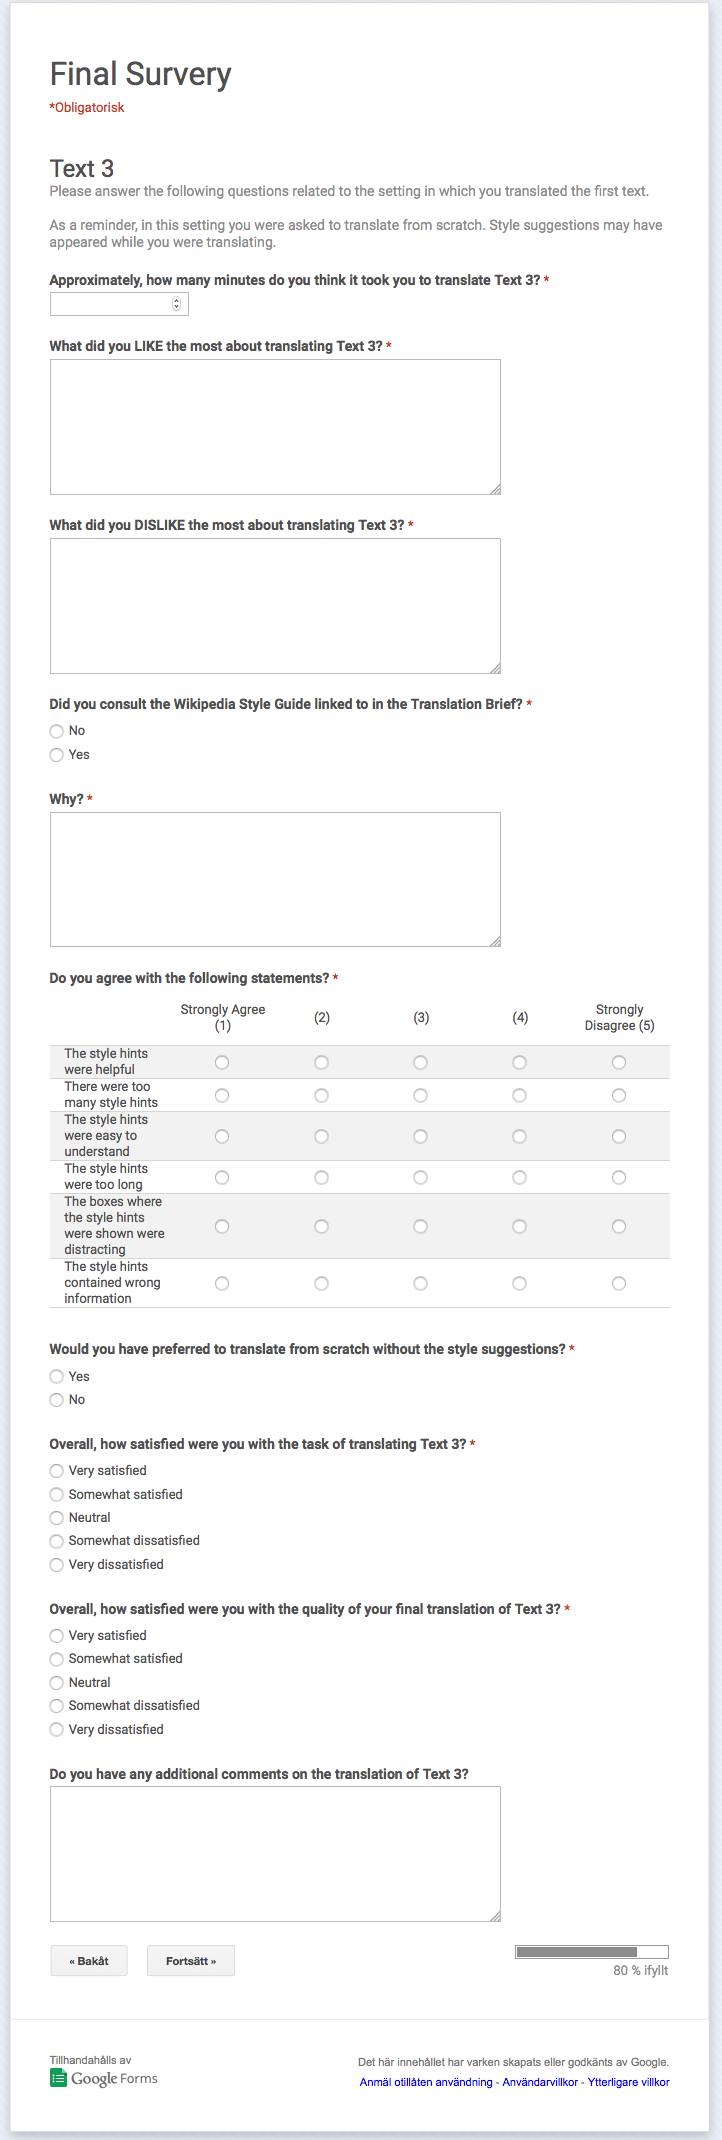
\includegraphics[height=\textheight]{img/final_questionnaire/final_4.png}
\caption{Final Questionnaire (Page 4)}
\end{figure}

\begin{figure}[h]
\myfloatalign
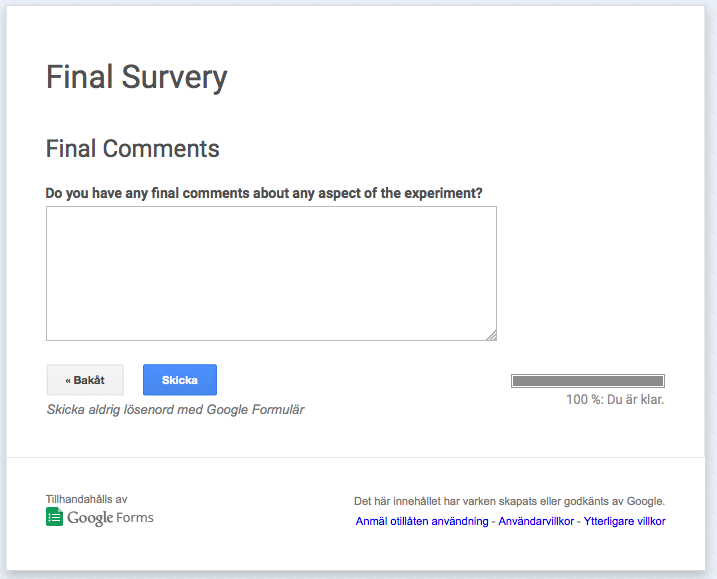
\includegraphics[width=\textwidth]{img/final_questionnaire/final_5.png}
\caption{Final Questionnaire (Page 5)}
\end{figure}
